%!TEX root = ../dissertation.tex
\chapter{Trigger}
\label{chap:trigger}

\indent Due to the large volume of data produce at the LHC, a efficient and robust triggering system is essential in deciding which events are potentially interesting and recorded for later study.  The ATLAS trigger system is divided into two levels in Run 2.  The first-level trigger (Level1 or L1 trigger) is hardware based and uses a subset of detector information to quickly reduce the rate of accepted events from the initial 40 MHz to 100 kHz.  Afterwards, the software based high-level trigger (HLT) further reduces the event rate to 1 kHz.  Any events passing the HLT are recorded by ATLAS for further reconstruction and offline analysis. \\

\indent Object reconstruct at the HLT is done only to the precision required by the executed trigger algorithms.  The online reconstruction algorithms tend to be less precise then the offline reconstruction algorithms described in chapter \ref{chap:reconstruction} but are significantly faster. \\

\indent A schematic showing the different ATLAS trigger components is given in figure \ref{fig:trigScheme}.  Only components relevant to the triggers used in this analysis will be discussed in detail.  Further detail can be found in \cite{Trigger2015}.

\begin{figure}[htb]
  \begin{center}
    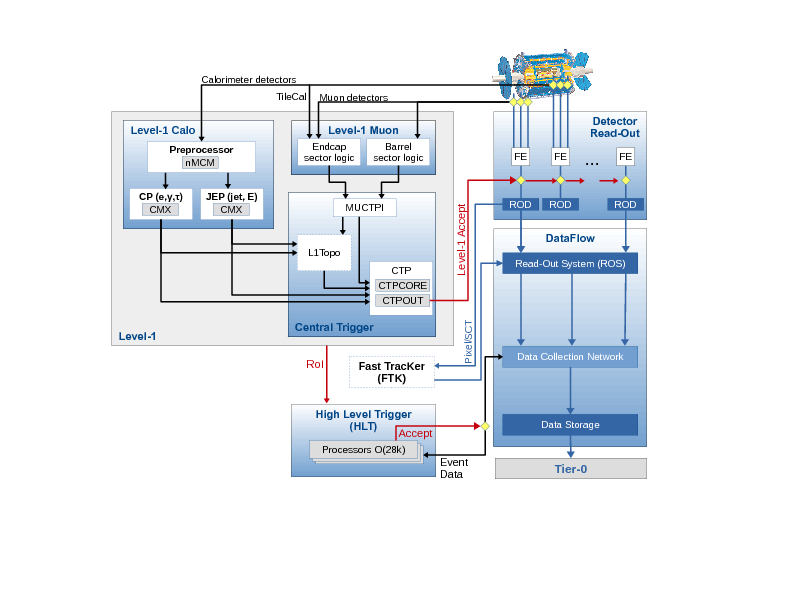
\includegraphics[width=0.80\textwidth]{figures/trigger/tdaq-schematic.png}\hspace{0.05\textwidth}
\end{center}
\caption{Schematic representation of the ATLAS trigger system and information flow.\cite{Trigger2015}}
\label{fig:trigScheme} 
\end{figure}

\indent We use the lowest un-prescaled $\met$ trigger in this analysis.  This corresponds to the {\sc HLT\_xe70\_mht\_L1XE50} trigger in 2015,  {\sc HLT\_xe90\_mht\_L1XE50} for 2016 data taking period A-D3, {\sc HLT\_xe100\_mht\_L1XE50} for the period D4-F1 and {\sc HLT\_xe110\_mht\_L1XE50} for period F2 and onward. The HLT trigger thresholds increase multiple times in 2015 and 2016 to accommodate the increasing instantaneous luminosity but all the triggers used are evaluated using the same algorithm.  All HLT triggers that we use are seeded by the L1\_XE50 trigger. \\

\indent A summary of the L1 and HLT $\met$ triggers used in this analysis is given in section \ref{sec:trig:L1Calo} to \ref{sec:trig:metHLT}\\

\section{Level 1 $\met$ trigger}
\label{sec:trig:L1Calo}

\indent The L1 $\met$ trigger is based on the vector sum of $E_T$ in the calorimeter and is part of the L1Calo trigger system \cite{L1Calo} shown in figure \ref{fig:trigScheme}.  The process starts with trigger towers in the electromagnetic and hadronic calorimeters.  Trigger towers are more corse then those used in offline reconstruction: Most are $0.1~\times~0.1$ in $\Delta\eta~\times~\Delta\phi$.  The trigger towers are calibrated at the electromagnetic energy scale (EM scale) which correctly reconstructs EM shower energy but underestimates hadronic showers.  \\

\indent These trigger towers are then built into jet elements composed of $2~\times~2$ EM trigger towers and combined with the $2~\times~2$ hadronic trigger towers directly behind the EM towers. The jet elements are then fed to the Jet/Energy-sum Processor (JEP).  The JEP calculates the global sums of $E_t$ and $\met$ by summing the $E_x$, $E_y$, and scalar $E_t$ of all jet elements.  If the total $\met = |- \sqrt{E_x^2+E_y^2}|$ is above a certain value the event passes the $\met$ trigger and is passed to the HLT.  The L1\_XE50 $\met$ trigger has a 50 $\gev$ threshold. \\

\section{HLT $\met$ trigger}
\label{sec:trig:HLT_MET}

\indent The reconstruction of $\met$ for the HLT also begins with identifying topo-clusters in the calorimeters.  Much like offline topo-clusters described in section \ref{sec:jet:reco}.  Seed cells with greater then $4\sigma$ signal over noise thresholds are first identified and neighboring cells with greater then $2\sigma$ thresholds are added.  Neighboring cells with greater then $2\sigma$ are continually added until no neighboring cell pass the $2\sigma$ threshold.  At this point, one final round of neighboring cells are added regardless of energy thresholds. \\

\indent Jet reconstruction and calibration are also similar to offline jet reconstruction described in section \ref{sec:jet:reco}.  Jets are reconstructed using the $\antikt$ algorithm from topo-clusters.  Jet calibration also follow the same basic offline procedure in section \ref{sec:jet:calib}. However, HLT jet calibration and offline calibration procedures do differ in many ways including different pile-up corrections, track-based correction and certain in-situ corrections.  Overall this leads to poorer jet resolutions at the HLT level.  Some of these corrections were added in 2016 to further improve the agreement between online and offline jet reconstruction.  Details can be found in \cite{Trigger2016}. \\

\indent The $\met$ is calculated directly by calculating the vector sum of the negative transverse momentum of all reconstructed jets.  Only contributions from the calorimeter is taken into account in the $\met$ calculation and muon tracks are not included.  This method of calculating the $\met$ from calibrated jets is referred to as missing $H_T$ (MHT).  \\

\indent We apply a 70, 90, 100, or 110 $\gev$ threshold to our HLT $\met$ trigger depending on the data taking period.  Trigger threshold increases over time because the instantaneous luminosity increases. \\

\indent Trigger turn on curves as a function of offline $\met$ can be seen in figure \ref{fig:trigTurnON}.  The poorer online $\met$ resolution leads to a more gradual turn on curve. \\

\begin{figure}[htb]
  \begin{center}
    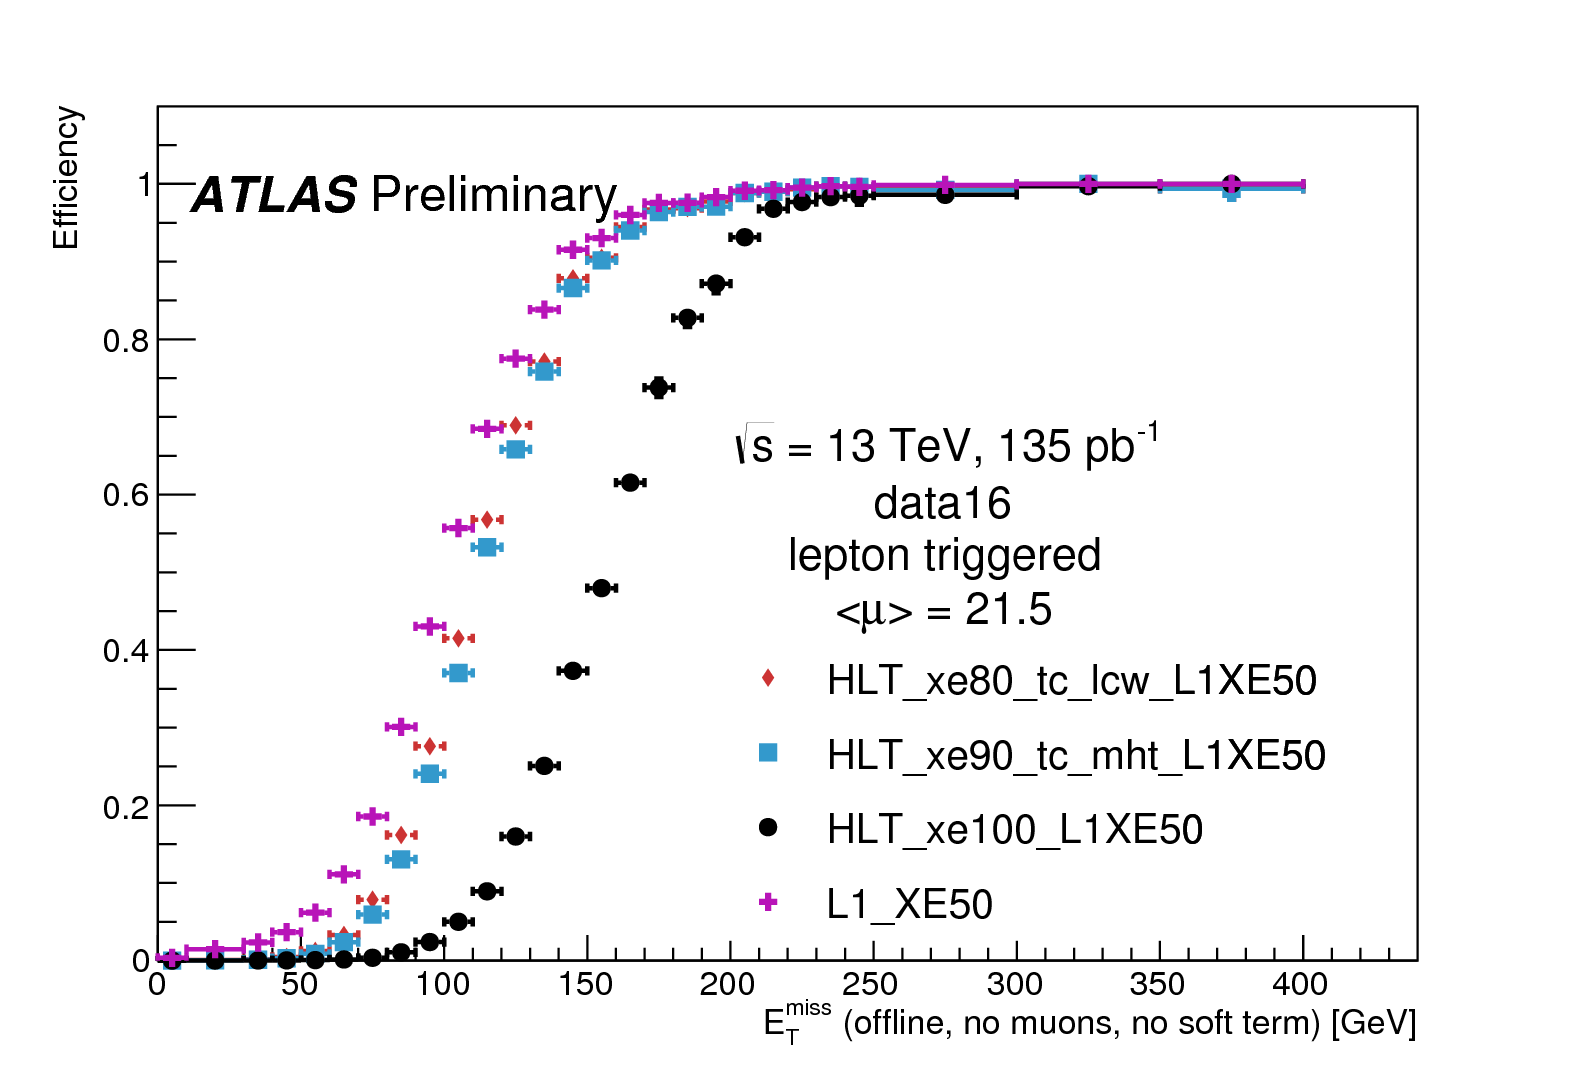
\includegraphics[width=0.65\textwidth]{figures/trigger/2016-05-16-UpdatedTurnOns.png}\hspace{0.05\textwidth}
\end{center}
\caption{ATLAS trigger turn on curves for MHT $\met$ triggers with several different thresholds. (Figure taken from \cite{Trigger2016})}
\label{fig:trigTurnON} 
\end{figure}

\section{Improvements to the $\met$ Trigger in Run 2}
\label{sec:trig:improvements}

\indent A significant improvement to pileup mitigation was made to the L1Calo trigger system for Run 2.\cite{Trigger2015}  The ATLAS Liquid Argon Calorimeter integrates its signal over a time window of $600$ ns.  This long time window corresponds to 24 bunch crossings.  Hence, energy deposition from collisions occurring in neighboring bunches (referred to as out-of-time pileup) will be registered as signal.  This results in a higher average signal amplitude (pedestal) in collisions at the beginning of a bunch train then those at the end of a bunch train.  \\

\indent The pedestal's dependence on bunch-crossing location was corrected offline but not at the trigger level in Run 1.  However in Run 2, a dynamic bunch-by-bunch pedestal correction was implemented at the trigger level.  This lead to a significant reduction in L1 $\met$ trigger rate as shown in figure \ref{fig:L1METImprove}. \\

\begin{figure}[htb]
  \begin{center}
    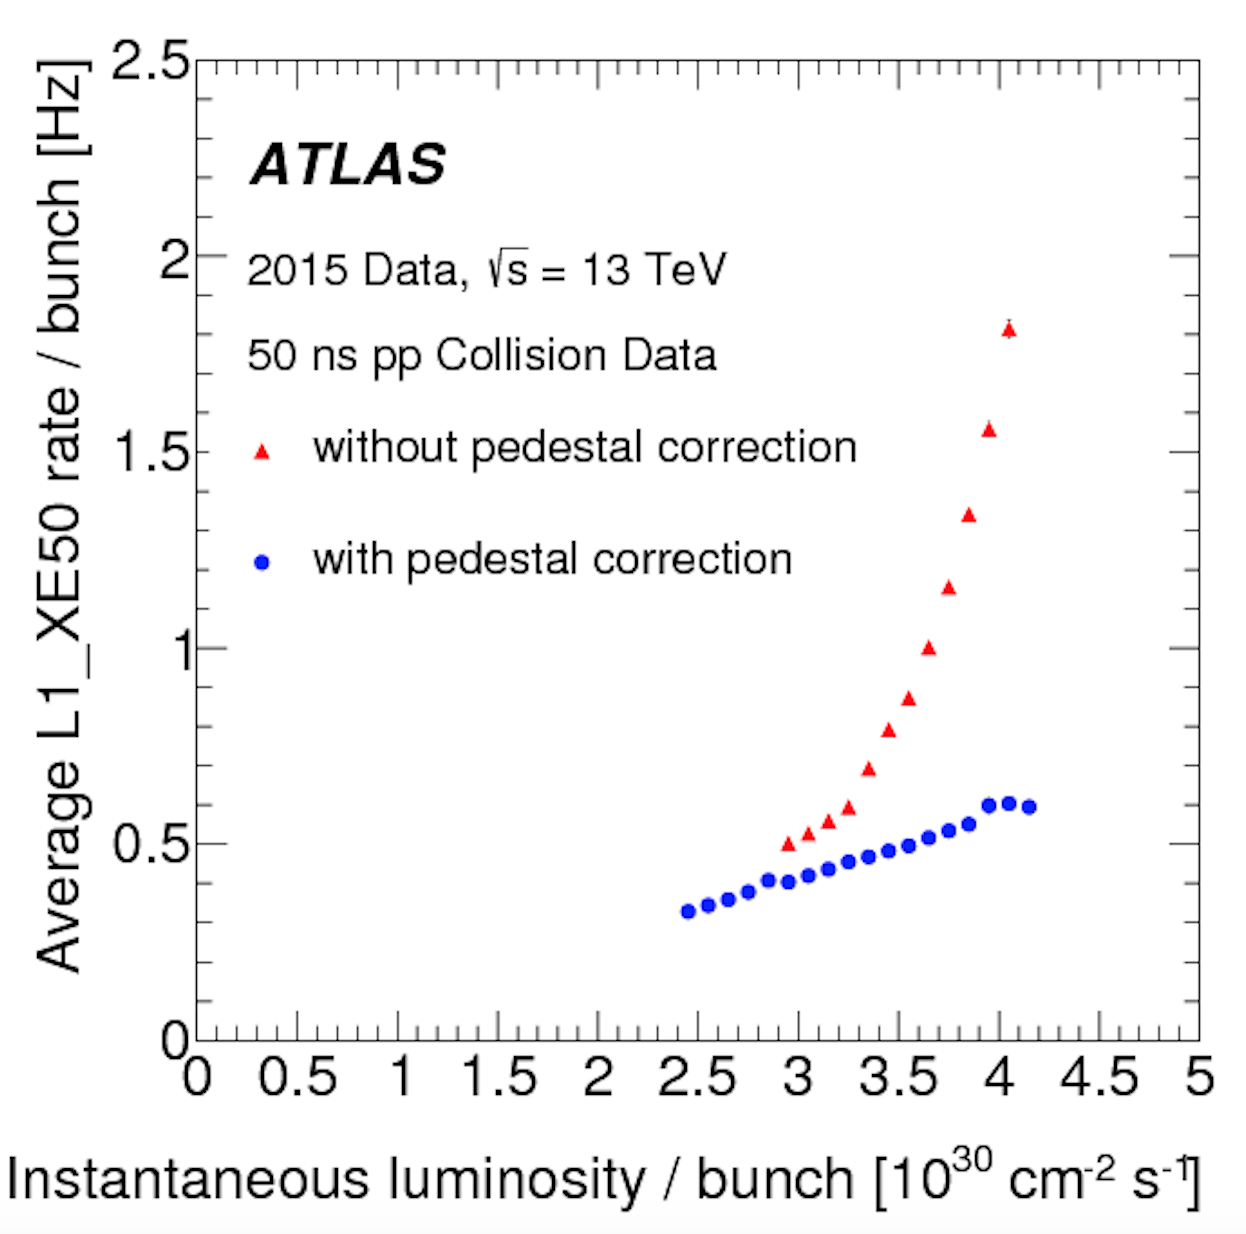
\includegraphics[width=0.65\textwidth]{figures/trigger/L1_XE50.png}\hspace{0.05\textwidth}
\end{center}
\caption{Improvement to the L1\_XE50 rate with new dynamic pedestal correction for out-of-time pileup.\cite{Trigger2015}}
\label{fig:trigScheme} 
\end{figure}

\indent This improvement to the LAr energy calibration also improves the jet energy calibration at the HLT.  This not only improves HLT $\met$ trigger performance but also improves the performance of other HLT calorimeter triggers such as those on total $E_T$. \cite{Trigger2016} \\